%\setlength{\parskip}{2.5pt plus 2pt minus 2pt}

\chapter*{Workshop Details}
\chead{Workshop Details}

%\addstarredchapter{About SPHERIC}
%\chaptermark{About SPHERIC}
\addcontentsline{toc}{chapter}{Workshop Details} \mtcaddchapter
\vspace{-5em}




\phantomsection
\addsec{Committees}\rhead{Committees}

\subsection*{Scientific Committee}\vspace{-1em}
%\addcontentsline{toc}{section}{Scientific Committee} 
\begin{itemize}
\item Prof. David Le Touz\'e (Ecole Centrale de Nantes, France)
\item Dr. Damien Violeau (Electricit\'e de France, France)
\item Dr. Nathan Quinlan (National Univ. of Ireland, Ireland)
\item Dr. Ben Rogers (University of Manchester, UK)
\item Prof. Stefano Sibilla (University of Pavia, Italy)
\item Dr. Jean-Christophe Marongiu (ANDRITZ Hydro, France)
\item Dr. Alex Crespo (Universidade de Vigo, Spain)
\item Dr. Andrea Colagrossi (INSEAN, Italy)
\item Dr. Xiangyu Hu (Technical University of Munich, Germany)
\item Prof. Rade Vignjevic (Brunel University of London, UK)
\item Prof. Thomas Rung (Technical University of Hamburg-Harburg, Germany)
\item Dr. Antonio Souto-Iglesias (Technical University of Madrid, Spain)
\item Dr. Renato Vacondio (University of Parma, Italy)
\item Dr. Matthieu De Leffe (Nextflow Software, France)
\item Prof. Moncho G\'omez-Gesteira (Universidade de Vigo, Spain)
\item Dr. Abbas Khayyer (University of Kyoto, Japan)
\item Prof. Walter Dehnen (University of Leicester, UK)
\item Dr. Raj Das (University of Auckland, New Zealand)
\item Prof. Robert A. Dalrymple (Johns Hopkins University , USA)
\item Prof. Alexis H\'erault (Conservatoire National des Arts et M\'etiers, France)
\item Prof. Joe Monaghan (Monash University, Australia)
\item Prof. Peter Eberhard (University of Stuttgart, Germany)
\item Prof. Moubin Liu (Peking University, China)
\item Dr Mehmet Yildiz (Sabanci University, Turkey)
\end{itemize}



\subsection*{Organizing Committee}
%\addcontentsline{toc}{section}{Organizing Committee} 
\subsubsection*{Chair}\vspace{-1em}
\begin{itemize}
\item Prof.   M. B. Liu, Peking University
\end{itemize}

\subsubsection*{Co-Chairs}\vspace{-1em}
\begin{itemize}
\item Prof.   H. F. Qiang, Xi'an Hi-Tech Institute, China
\item Prof.   A. M. Zhang, Harbin Engineering University, China
\item Prof.   L. Zou, Dalian University of Technology, China
\item Prof.   D. A. Hu, Hunan University, China
\item Prof.   F. Xu, Northwestern Polytechnical University, China
\item Prof.   Z. R. Li, Wenzhou University, China
\end{itemize}


\newpage
\phantomsection
\addsec{Keynote Speakers}
\rhead{Keynote Speakers}
\phantomsection
\subsection*{Prof.  David Le Touzé}\label{David}
\textit{Ecole Centrale Nantes}\\
\textit{Deputy Head, LHEEA research dept. (ECN and CNRS)}\\
\textit{Head, H2I research group of LHEEA}\\
\textit{Head, Centrale Nantes - Bureau Veritas Chair}\\
\textit{Head, IRT Jules Verne SimAvHy Chair}

\textbf{Title}: Smoothed Particle Hydrodynamics, fact checking: from theory to applications

%\textbf{Abstract}: An overview of the Smoothed Particle Hydrodynamics applied to free-surface and interface flows is provided in the talk, under the form of fact checking. The complex links between the Lagrangian feature of the method, the smoothed and discretized operators, the modeling of physical terms and boundary conditions, on the one hand, and the conservation, convergence and accuracy of the method, on the other hand, are discussed. The links between the physical modeling of free-surface conditions and incompressibility, and the time solving and HPC implementation of the method are also explored. This current understanding of the SPH method permits to highlight the current successful SPH schemes, their accuracy, efficiency, limitations and target types of applications. A set of example successful industrial engineering applications is presented. The interest and feasibility of coupling to other methods is also highlighted.

\textbf{Bio}: Prof. David LE TOUZÉ is 40 years old. He got his MSc in Hydrodynamics and Ocean Engineering from Ecole Centrale Nantes (Nantes, France) in 2000. Ecole Centrale Nantes is a highly competitive French « Grande Ecole » which awards MScs and PhDs only. He then got his PhD with honors in 2003 from the same institute, whose topic was modeling gravity wave generation and propagation by spectral methods. He spent 2 years of post-doc at CNR-INSEAN (Rome, Italy) in 2004-05 where he started working in SPH. He came back to Ecole Centrale Nantes in 2006 and became Assistant Professor in 2007, Associate Professor in 2010 and Full Professor in 2012. His researches revolve mainly around free-surface flows. He is leading since 2012 a research group on Hydrodynamics, Interfaces and Interactions (H2i) which counts 8 professors and researchers, 14 PhD students, and 6 post-docs. His current research topics cover different numerical methods and techniques: SPH (Smoothed Particle Hydrodynamics), incompressible (OpenFOAM) and weakly-compressible (WCCH) Finite Volumes, Adaptive Mesh Refinement (AMR), Immersed Boundary Method (IBM), Vortex Method (DVH), Lattice-Boltzmann Method (LBM). He is also working on different method couplings: potential (waves) to Navier-Stokes Finite Volume Method for wave-structure interactions, SPH to Finite Element Method (FEM) for fluid-structure interaction, SPH to Finite Volume Method for efficient solutions of complex flows. Main applications of his research are in the fields of marine engineering (many naval, offshore and marine renewable energy topics), automotive (aquaplaning, gear boxes), aeronautics (ditching) and health (cardio-vascular flows). He is currency leading 7 industrial projects (over 5M contracts). He is the author of 30+ journal publications, with a google h-index of 22. He is also Deputy Head of his research department (LHEEA, 140 staff) which is a joint research unit between Ecole Centrale Nantes and CNRS.

\phantomsection
\subsection*{Prof.  J. S. Chen}\label{Chen}
\textit{William Prager Chair Professor, Structural Engineering Department, Director, Center for Extreme Events Research, University of California, San Diego}

\textbf{Title}: An Implicit Gradient Reproducing Kernel Particle Method: Theory and Applications

%\textbf{Abstract}: High strain rate events such as projectile penetration and blast often result in fragmentation, complex contact conditions, and severe material damage. The Reproducing Kernel Particle Method (RKPM) relies on nodal integration to yield a pure point-based method for effective simulation of these events, however stability of nodal integration is difficult to achieve without upsetting computational efficiency or introducing user-tuneable parameters. In this work, a naturally stabilized nodal integration method is formulated under a strain-smoothing framework, and a variational consistency correction for nodal integration is introduced to ensure optimal convergence. Taylor expansion of nodal strains in conjunction with implicit gradients yields high computational efficiency, with stabilization constants naturally arising as moments of inertia of nodal domains. The method is cast under a strain smoothing framework to achieve additional stability in extreme event modelling, with the benefit of further enhancing computational efficiency. Simulation of blast and penetration events will be presented to demonstrate the effectiveness of the proposed method.

\textbf{Bio}: J. S. Chen earned his undergraduate degree from National Central University (1978-1982) in Taiwan, and received master's (1986) and Ph.D. (1989) from Northwestern University. He worked in GenCorp's Research Division from 1989 to 1994. From 1994 to 2001, he held a faculty position in the Mechanical Engineering Department of The University of Iowa before moving to UCLA in 2001, where he served as the Chair of Civil \& Environmental Engineering Department from 2007 to 2012. He was the Chancellor's Professor in the Civil \& Environmental Engineering Department at UCLA and also Professor of Mechanical \& Aerospace Engineering Department and Mathematics Department. In 2013, he joined the Structural Engineering Department of UCSD as the inaugural holder of the William Prager Endowed Chair. He also is the director of the Center for Extreme Events Research at the Jacobs School of Engineering at UC San Diego.




\newpage
\phantomsection
\addsec{Conference Venue}\rhead{Conference Venue}
The SPHERIC Beijing 2017 will be held at Peking University, Beijing, China.
\begin{itemize}
\item Address: No.5 Yiheyuan Road Haidian District, Beijing, P.R.China 
\item Tel:  +86 1062 766 982
\item Website: \url{http://ocean.pku.edu.cn/SPHERIC_Beijing/index.php.htm}
\end{itemize}

\phantomsection
\addsec{Accommodation}
\textbf{For participants outside China}, the committee has reserved rooms at \textbf{ZhongGuanYuan Global Village PKU} at discounted prices. It should be noted that the registration fee does not include accomodation. All of the hotels below include breakfast and wifi access. 
\begin{itemize}
\item Address: No.126 ZhongGuanCun North Street, Haidian District, Beijing, China
\item Tel:  +86 10 62752288
\item Website: \url{http://www.pkugv.com}
\end{itemize}

\phantomsection
\addsec{Transportation Information}
TAXI Taxi is the most convenient transportation to the University from the airport. As the Capital Airport is located 40 km northeast from the campus, it will cost you around 100-130 RMB (expressway fee of 15 RMB included) to get to the university from the airport. It takes approximately 1-1.5 hours to arrive at PKU from the airport, depending on the traffic.

Getting to PKU from the Airport BUS You may also first travel to ZhongGuanCun via the airport shuttle bus and then take a taxi from ZhongGuanCun.

\begin{tikzpicture}[font=\footnotesize]
\node(zgc)[shape=rectangle,draw,minimum height=3em] at (0,0){Zhongguancun};
\node(cia)[shape=rectangle,draw,text width=8em,text centered, minimum height=3em] at (-6.85,0){Beijing Capital\\ International Airport};
\node(pku)[shape=rectangle,draw,text width=7em,text centered, minimum height=3em] at (6.85,0){Peking University};
\draw[->,>=stealth'] (cia)--(zgc) node[midway,above]{approx. 50 min} node[midway,below]{Airport Bus};
\draw[->,>=stealth'] (zgc)--(pku) node[midway,above]{approx. 6 min} node[midway,below]{Taxi};
\end{tikzpicture}


You may also take the subway. Take the Line `Airport Express' from Terminal 2 or Terminal 3, and transfer to Line 10 at the `Sanyuanqiao' station, and then transfer to the Line 4 at `Haidian Huangzhuang' station, and finally get off at `The East Gate of Peking University' station.

\begin{tikzpicture}[font=\footnotesize]
\node(cia)[shape=rectangle,draw,text width=8em,text centered, minimum height=3em] at (-6.85,0){Beijing Capital\\ International Airport};
\node(syq)[shape=rectangle,draw,text width=5em,text centered, minimum height=3em] at (-1.5,0){Sanyuanqiao Station};
\node(hhz)[shape=rectangle,draw,text width=8em,text centered, minimum height=3em] at (2.5,0){Haidian Huangzhuang Station};
\node(pku)[shape=rectangle,draw,text width=7em,text centered, minimum height=3em] at (6.85,0){East Gate of Peking University};
\draw[->,>=stealth'] (cia)--(syq) node[midway,above]{18 min} node[midway,below]{Airport Express};
\draw[->,>=stealth'] (syq)--(hhz) node[midway,above]{24 min} node[midway,below]{Metro};
\draw[->,>=stealth'] (hhz)--(pku) node[midway,above]{4 min} node[midway,below]{Metro};
\end{tikzpicture}


\newpage
\phantomsection
\addsec{Registration/Information Desk}\rhead{Registration/Information desk}
The registration desk at Room 104 in the Peking University Overseas Exchange Center, will be open from 8:30‐18:00 on Tuesday 17th October.

\phantomsection
\addsec{Instructions for Presenters}
\begin{itemize}
\item According to SPHERIC Workshop Presentation Style, each presenter will have 13 minutes strictly to present their work, followed by the successive presenter.  After all the presentations in a specific session, all the presenters will be asked to stand in front of the conference room and answer possible questions in a Group.
\item There is no need to explain the very basics of SPH to an SPH specialist audience, and please emphasize what is new and novel in method or application.
\end{itemize}

\phantomsection
\addsec{SPH Training Day}

Supplementary to the workshop, an SPH training day will be offered on 17 October 2017. The training is most suitable for researchers who are familiar with the principles of SPH but are beginning their work in the field. More experienced SPH developers and users may find that the training day is a useful opportunity for sharing insights and ideas. The SPH training day will also take place at the Peking University.

\phantomsection
\addsec{Other Tips}
\textbf{Free wifi connection}: TBD, EDUROAM is also available.

\textbf{Name tags}: Name tags are required for entry to all conference events. Please wear them at all times.



%\newgeometry{left=0.8in,right=0.8in,top=0.8in,bottom=0.8in}



\newpage\phantomsection
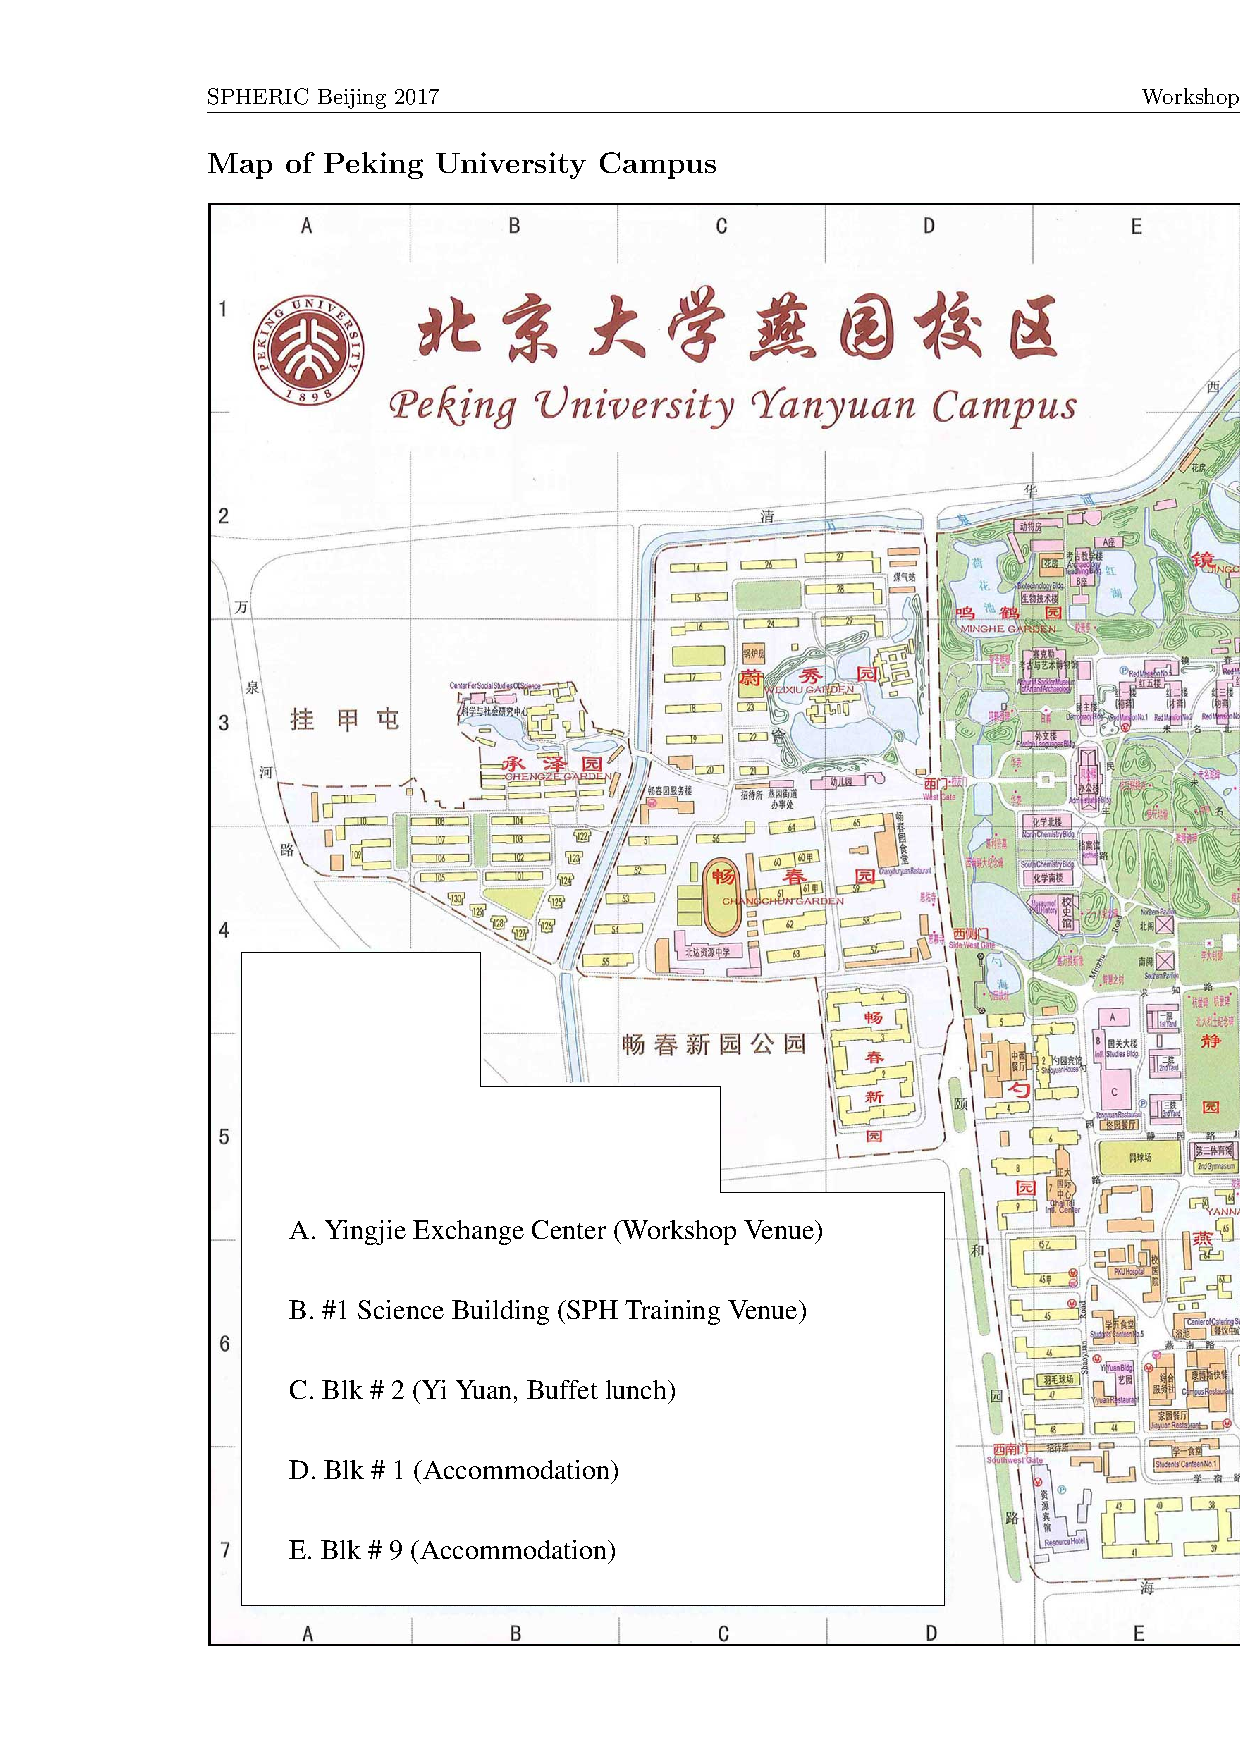
\includepdf[pages=1,pagecommand={\thispagestyle{plain}\addcontentsline{toc}{section}{Map of Peking University Campus}}]{figures/PKU2page.pdf}
\includepdf[pages=2,pagecommand={\thispagestyle{plain}}]{figures/PKU2page.pdf}



%\newpage\phantomsection
%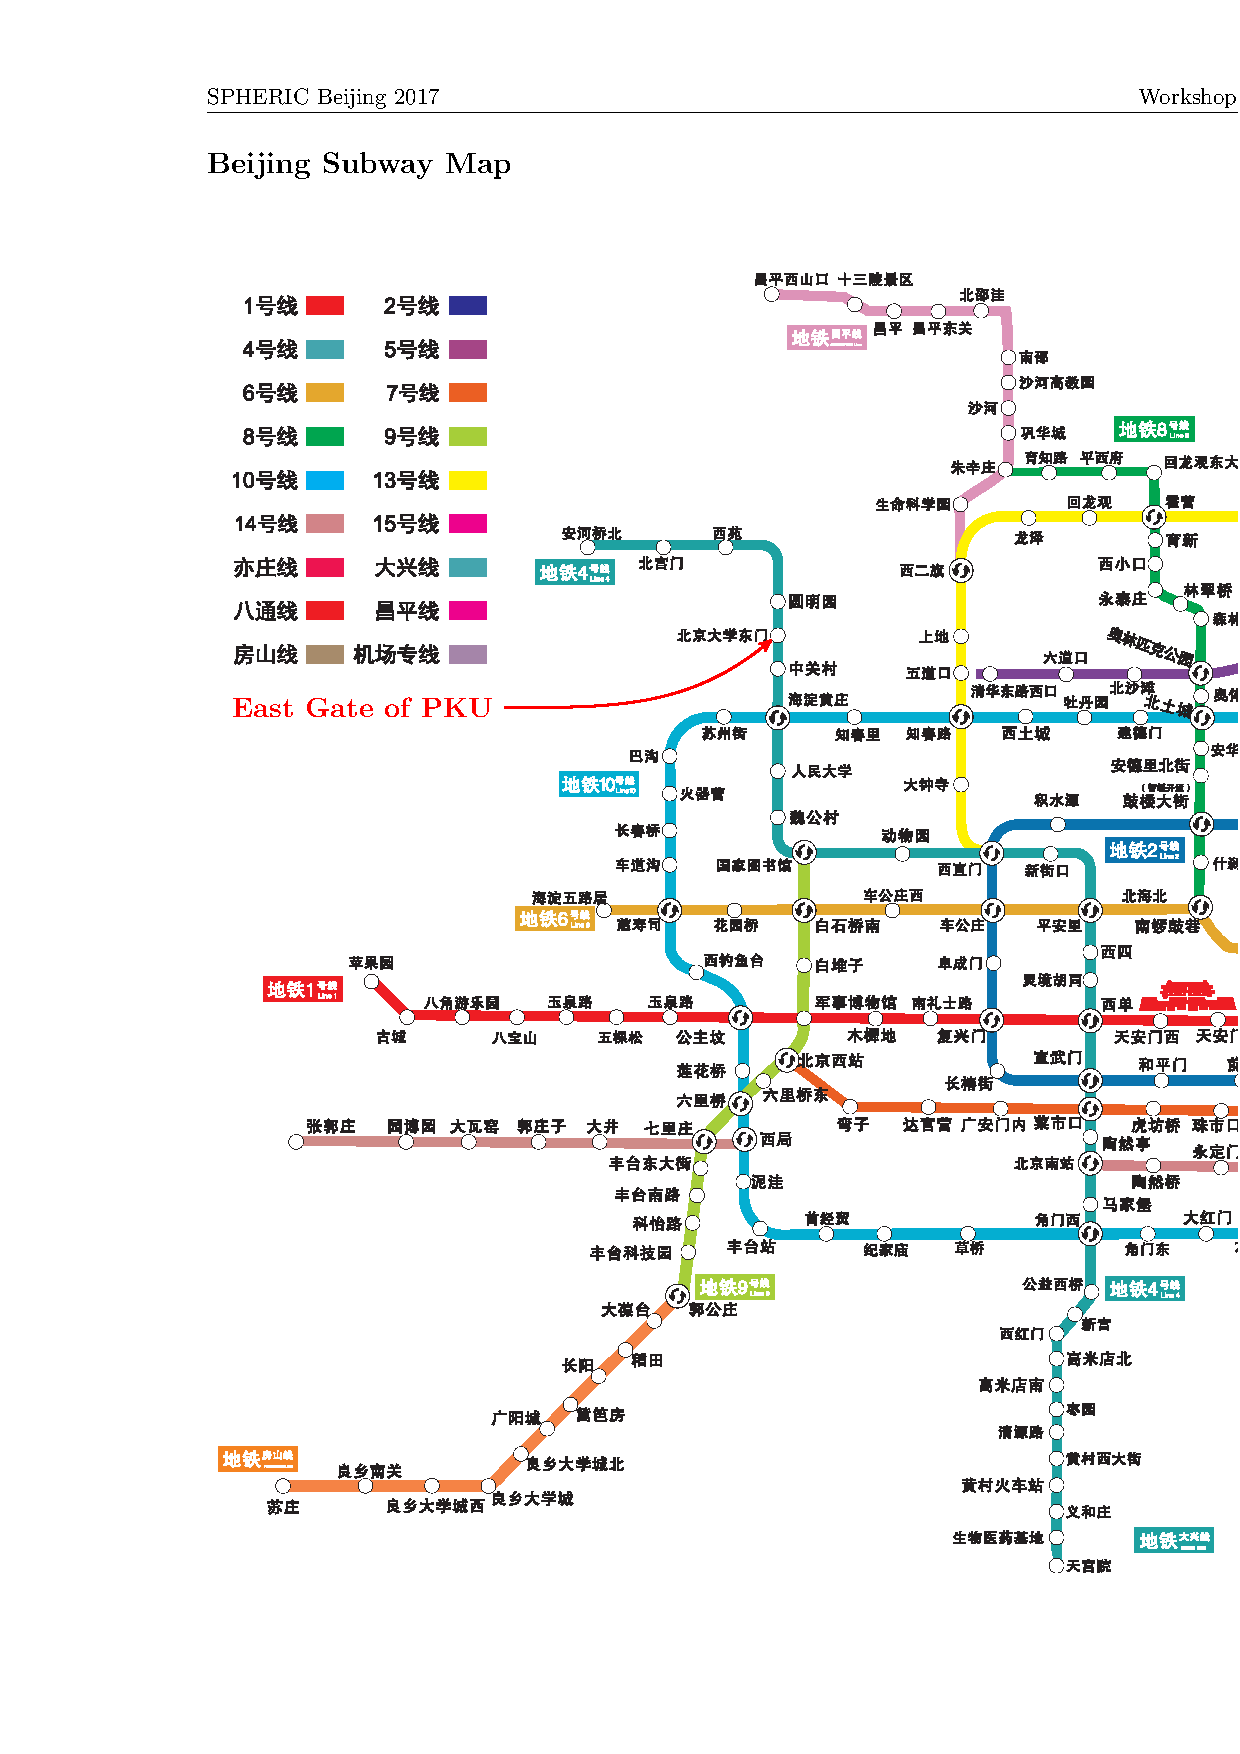
\includepdf[pages=1,pagecommand={\thispagestyle{plain}\addcontentsline{toc}{section}{Beijing Subway Map}}]{figures/subway2page.pdf}
%\includepdf[pages=2,pagecommand={\thispagestyle{plain}}]{figures/subway2page.pdf}


%\begin{landscape}
%\pagestyle{plain}
%\fancyhead{}
\lhead{SPHERIC Beijing 2017}\rhead{Beijing Subway Map}
\phantomsection
\addsec{Beijing Subway Map}
\begin{center}
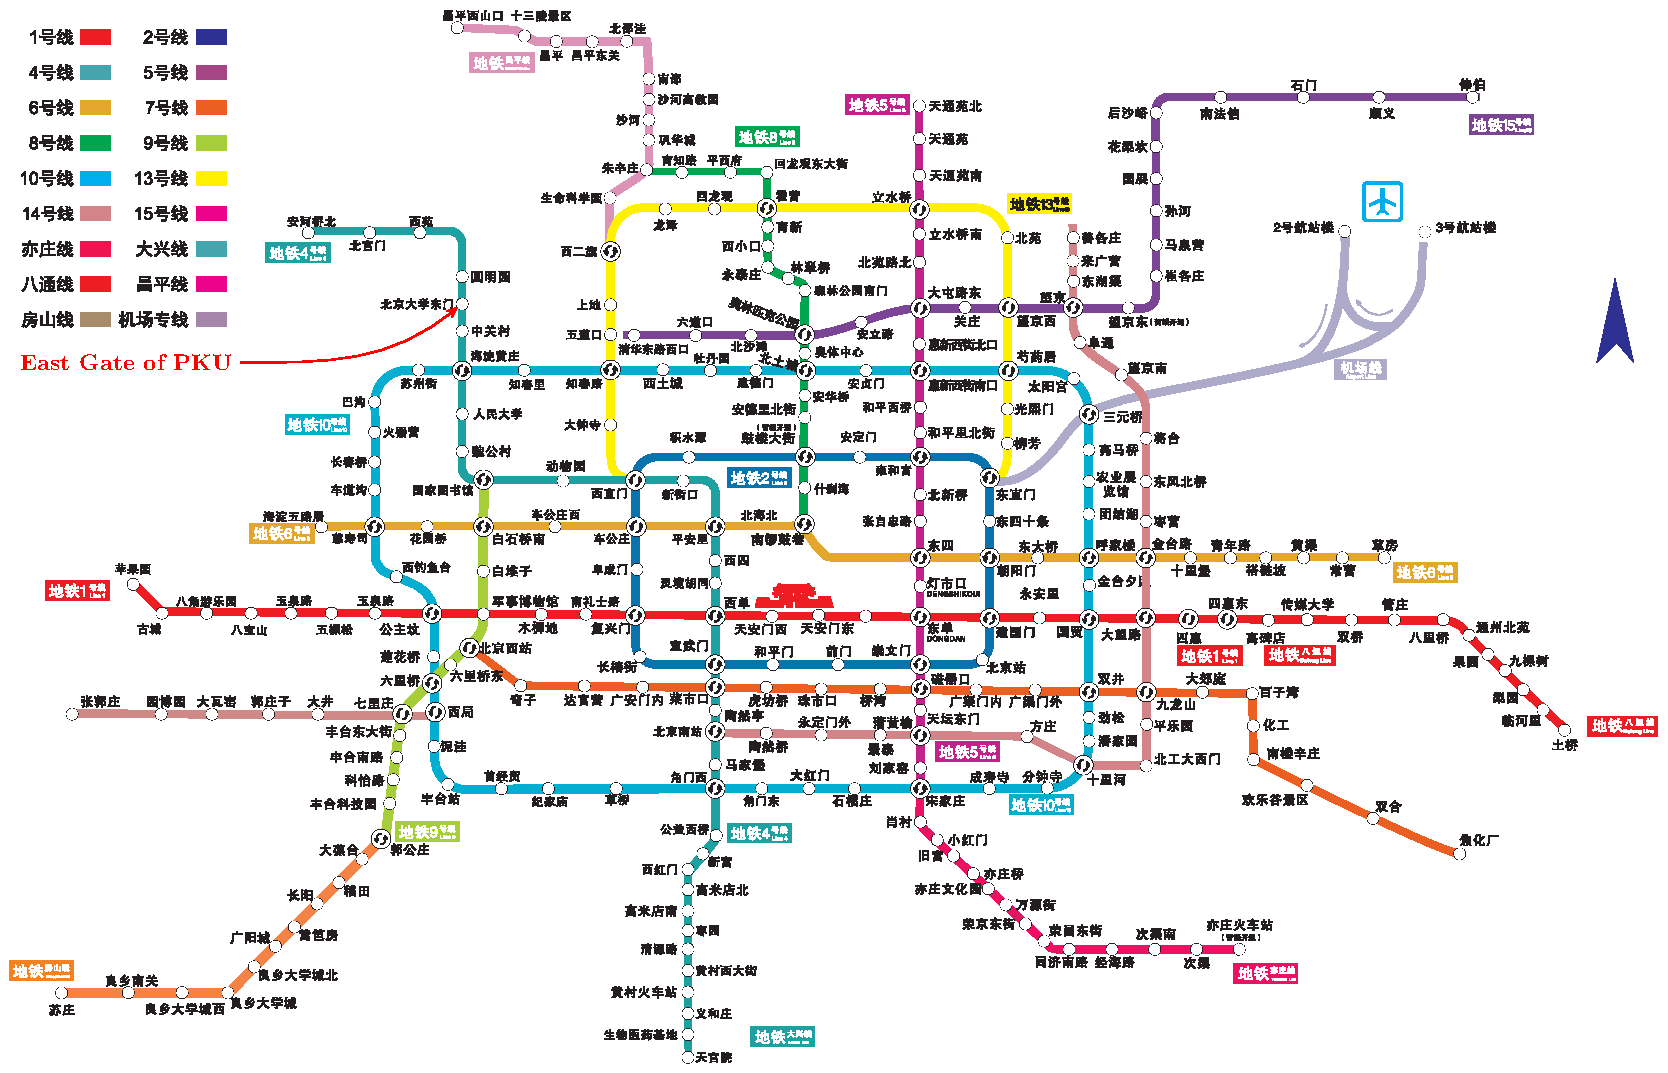
\includegraphics[angle=90,width=0.61\textheight]{subway.pdf}
\end{center}
%\end{landscape}





\newgeometry{left=0.8in,right=0.8in,top=1in,bottom=0.7in}
\newpage
\pagestyle{fancy}
\fancyhead{} 
\lhead{SPHERIC Beijing 2017}
\chead{Workshop Details}
\rhead{Floor Plan of Yingjie Exchange Center}
\phantomsection
\addsec{Floor Plan of Yingjie Exchange Center, Peking University}
\begin{center}
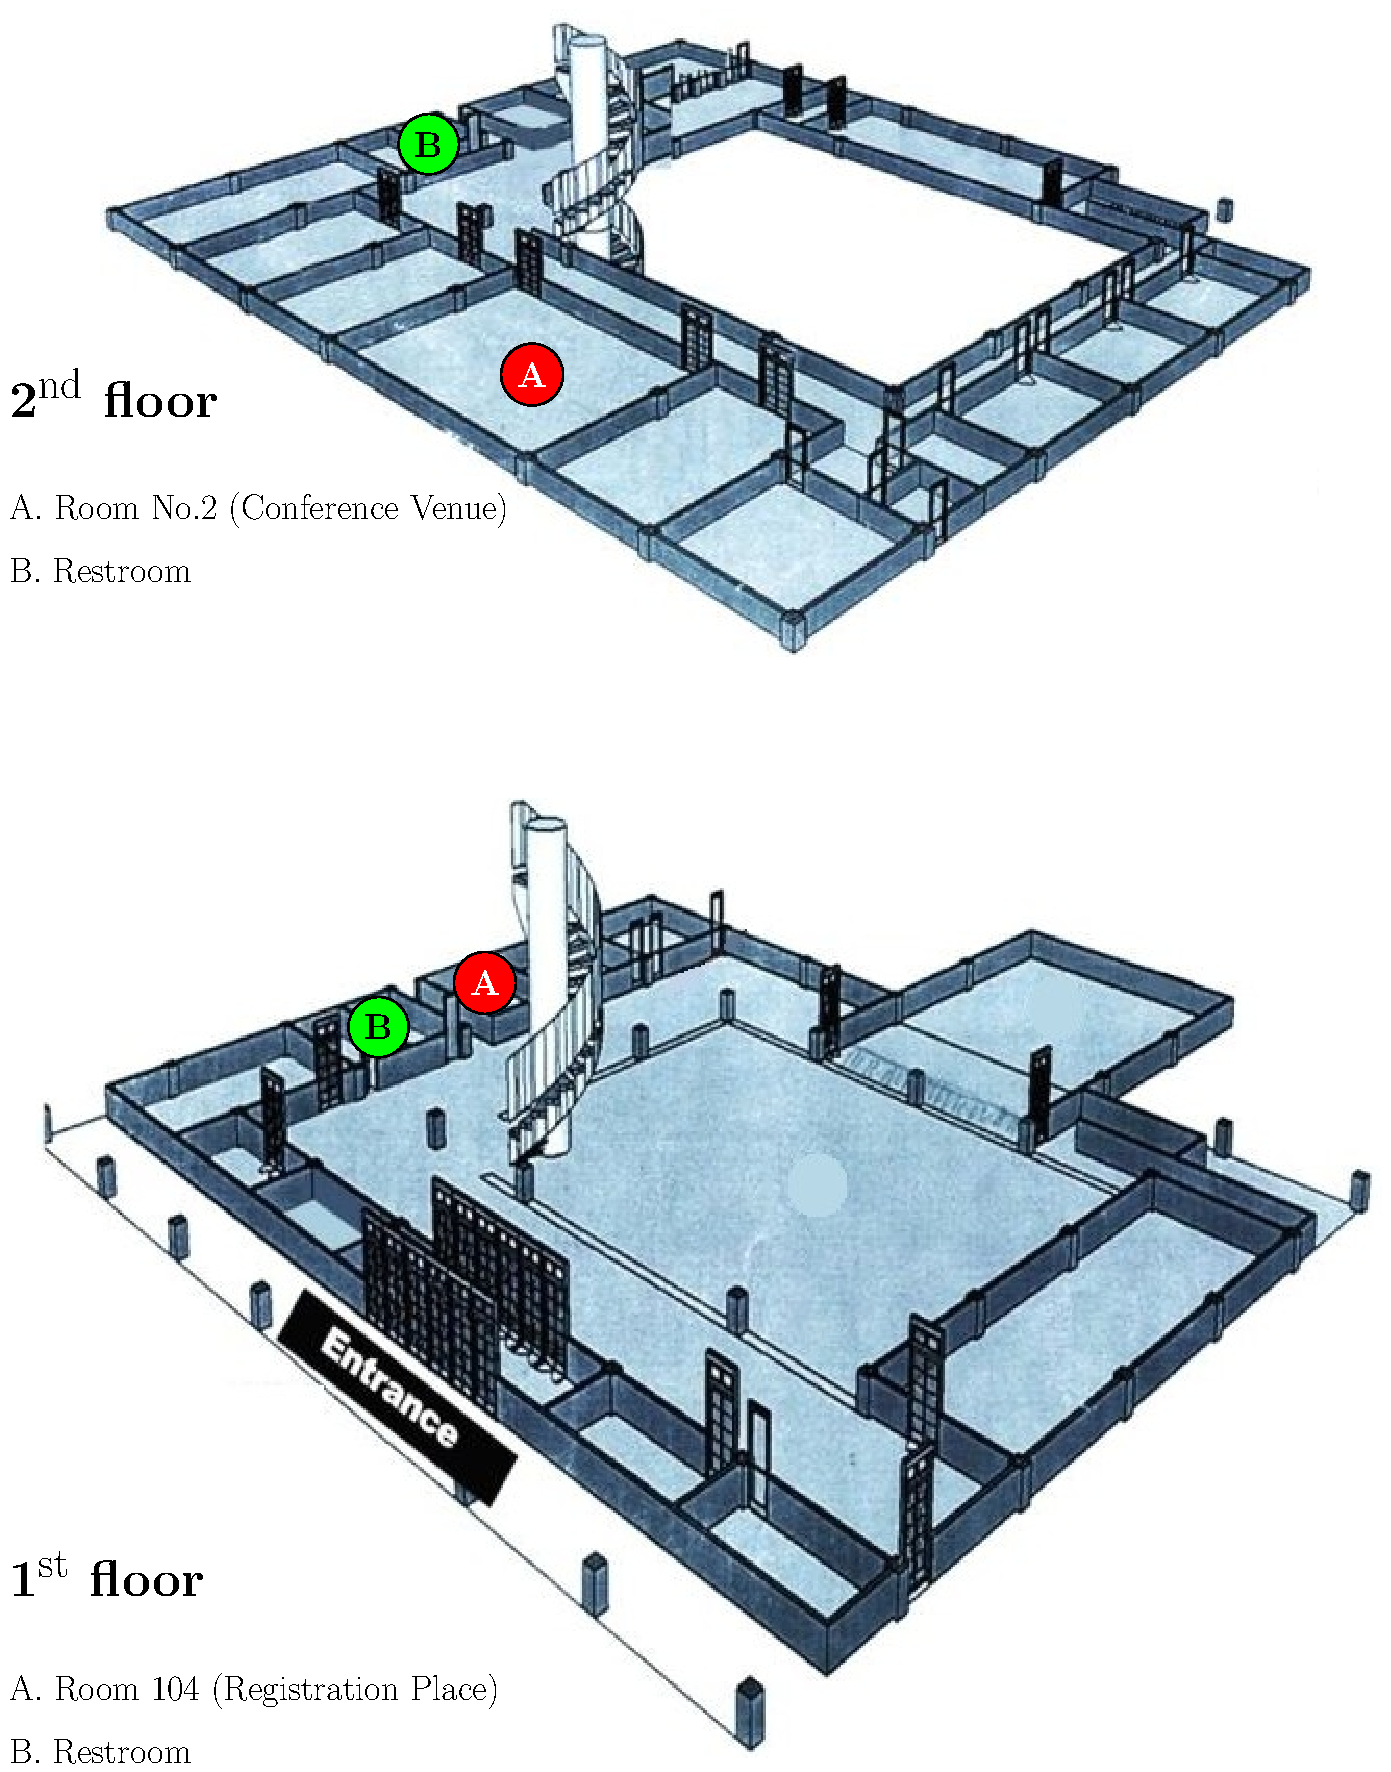
\includegraphics[width=\textwidth]{YJ.pdf}
\end{center}











